% !TeX spellcheck = en_US
% !TEX encoding = UTF-8 Unicode
\documentclass[12pt,a4paper, twocolumn]{article}
\usepackage[T1]{fontenc}
\usepackage{fontspec}
\usepackage{amsmath}
\usepackage{amssymb}
\usepackage{graphicx}
\usepackage{fancyhdr}
\usepackage{lastpage}
\usepackage[left=1.50cm, right=1.50cm, top=1.50cm, bottom=1.50cm, includeheadfoot]{geometry}
\usepackage{subfigure}
\usepackage{wrapfig}
\usepackage{mathtools}
\usepackage[nottoc, numbib]{tocbibind}
\usepackage{tabularray}
\usepackage{svg}

% \setmainfont{Verdana}

\newcommand{\Mnewline}{\\[0.2cm]}

\usepackage[pdfauthor={Nikolaos Stylianou},
pdftitle={Semester Project},
pdfcreator={TeX},
pdfsubject={ECE 494 - Processor Design}]{hyperref}

\hypersetup{
	colorlinks,
	citecolor=blue,
	filecolor=black,
	linkcolor=black,
	urlcolor=blue
}

\pagestyle{fancy}
\fancyhf{}
\fancyhead[L]{ECE 494 - Processor Design}
\fancyfoot[R]{Page \thepage \hspace{1pt} of \pageref*{LastPage}}
\renewcommand{\footrulewidth}{0.4pt}% Line at the footer visible

\fancypagestyle{first_page}{
\fancyhf{}
\fancyfoot[R]{Page \thepage \hspace{1pt} of \pageref*{LastPage}}
\renewcommand{\headrulewidth}{0pt}
\renewcommand{\footrulewidth}{0.4pt}
}

\title{\vspace{-0.5cm}Semester Project \Mnewline \normalsize{Architectural exploration of low-pass FIR filters using MATLAB HDL Coder}}
\author{Student: Nikolaos Stylianou \Mnewline
	ΑΕΜ: 2917 \Mnewline
	Course: ECE 494 - Processor Design \Mnewline
	
\includegraphics[scale=0.25]{Images/uth-logo.png}}
\date{\today \vspace{2cm}}

\begin{document}
	
\maketitle
\thispagestyle{first_page}
\vspace{3cm}
	
\tableofcontents

\newpage

% \input ta pages poy 8a graftoyn
\section{Introduction}

A low-pass FIR (\textit{Finite Impulse Response}) filter is a type of digital filter used in signal processing to attenuate or remove high-frequency components from a signal, allowing only low-frequency components to pass through. FIR filters are characterized by their impulse response, which is a finite duration sequence of coefficients.
The basic operation of a low-pass FIR filter involves convolving the input signal with the impulse response of the filter. The filter coefficients determine the filter's frequency response, and specifically in a low-pass filter, they emphasize the passage of low-frequency signals and suppress higher frequencies
The design of a low-pass FIR filter involves determining the appropriate filter order (length) and selecting the filter coefficients. The filter order determines the length of the filter's impulse response and affects the sharpness of the filter's frequency cutoff. Higher filter orders generally result in steeper roll-off characteristics but require more computational resources.

% For this project, my main point of interest is exploring the architecture of an FIR filter with the following characteristics:
For this project, I will be focused in exploring the architecture of an FIR filter with the following characteristics:

\begin{itemize}
    \item Sampling frequency: 46 kHz
    \item Pass frequency: 8 kHz
    \item Stop frequency: 9.6 kHz
    \item Number of coefficients:
    \begin{itemize}
        \item Minimum coefficients possible
        \item 20 coefficients
        \item 30 coefficients
    \end{itemize}
    \item Arithmetic:
    \begin{itemize}
        \item Single precision floating point
        \item Fixed point 24 bits
        \item Fixed point 16 bits
        \item Fixed point 8 bits
    \end{itemize}
    \item Optimizations:
    \begin{itemize}
        \item 1 stage multiplier pipelining
        \item 2 stage multiplier pipelining
        \item Multiplier-less using CSD
        \item Distributed Arithmetic
    \end{itemize}
\end{itemize}

The implemented filter has a magnitude response as figure~\ref{fig:fir_mag_response} shows.

\begin{figure}
    \centering
    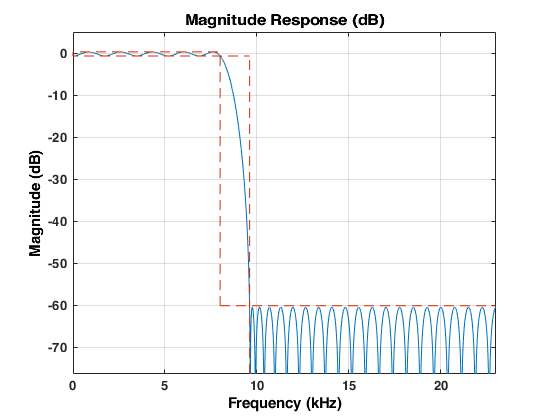
\includegraphics[width=0.4\textwidth]{Images/fir_minimum_mag_response.png}
    \caption{FIR magnitude response}
    \label{fig:fir_mag_response}
\end{figure}
\section{Filter Creation}
Before creating any HDL code, the filter has to be normally implemented in MATLAB.
Using \verb|designfilt| command, every parameter of the filter is filled with the help of GUI. We call this function 3 times, one for each different order of filter, thus creating 3 different FIR filters.
\begin{figure}[htpb]
    \centering
    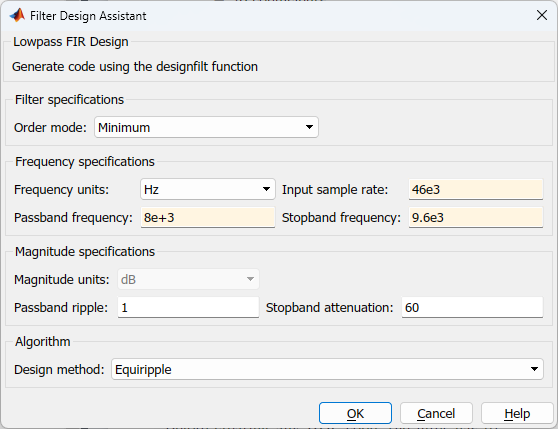
\includegraphics[width=0.4\textwidth]{Images/matlab_filter_design_assist_tool.png}
    \caption{MATLAB's design assist tool for creating lowpass FIR filters}
    \label{fig:matlab_filter_design_assist_tool}
\end{figure}
Using \verb|fvtool|, all three filters can be compared and be checked for compliance. 

For HDL Coder to work, all filters must be designed by \verb|fdesign.lowpass()| and \verb|design()| functions, thus all filters created above must be re-created. The first function creates the specification for each filter containing useful information such as passband/stopband frequency, sample rate, etc. In order to actually create the filter, \verb|design()| function has to be called and it returns \verb|dsp.FIRFilter| data type, meaning that the wanted filter is successfully created. Note that, we make use of two specific toolboxes provided by Mathworks, called \emph{DSP System Toolbox} and \emph{DSP HDL Toolbox} that provide those "easy" methods of creating filters alongside with optimizations like pipelining, CSD and others needed for this project. 

After each filter is created, \verb|fdhdltool| has to be called with filter specifications and numeric type needed as arguments.
Every aspect of the generated filter can be tuned from there such configuring architectures, multiplier pipelining, test bench generator and more. This task has to be executed for each implemented filter.

\begin{figure}[htbp]
    \centering
    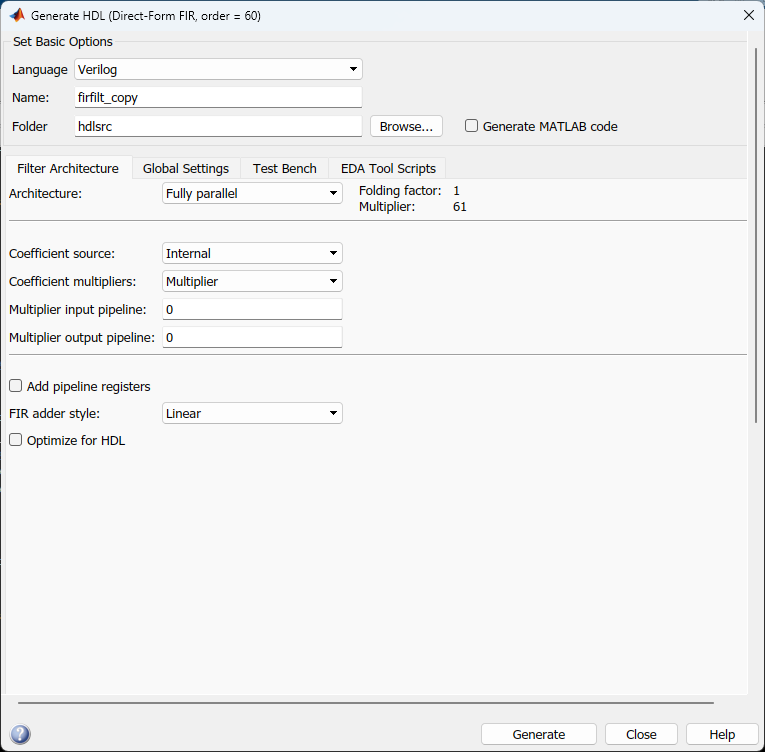
\includegraphics[width=0.4\textwidth]{Images/matlab_create_hdl.png}
    \caption{MATLAB's tool for creating HDL filters.}
    \label{fig:matlab_create_hdl}
\end{figure}

\section{Filter Synthesis}

Once creating every filter with its own configuration, each HDL file has to be synthesized and/or implemented in order to compare each architecture.
For this process, Xilinx Vivado seems to be the best option to use as other great EDA tools like Synopsys and Cadence suites weren't available. Since I'm using Vivado, I should as well target an FPGA that might have access such as the \href{https://www.xilinx.com/products/boards-and-kits/1-8dyf-11.html}{Zedboard}. Zedboard isn't a very big FPGA in terms of memory size, but, hopefully, it might be able to implement some filters at the end.

\subsection{Importing MATLAB HDL files}
In Vivado, a new project is created for each filter architecture. Files are imported using the standard GUI procedure while also adding constraints for the target device mentioned above.
MATLAB produces source HDL and test-bench for each filter created.
% !TeX spellcheck = en_US

\section{Filter Comparison}

\subsection{Architectural differences}
The main difference of each pack of filters is the architecture itself.
Using a standard multiplier, the filter coefficients are multiplied with the input samples using multipliers. The output is obtained by summing the products of the coefficients and input samples. This architecture is straightforward and produces accurate results but can be resource-intensive in terms of hardware implementation.

The second implementation is by using factored CSD., This is a technique used to reduce the number of partial products required for multiplication by decomposing the coefficients into a sum of powers of two. This architecture employs a combination of shifters and adders to implement the multiplication operation. The output is obtained by accumulating the partial products. Factored CSD reduces hardware complexity and power consumption compared to the multiplier architecture, but it may introduce some additional round-off errors due to approximation.

The last architecture used in this project is called Distributed Arithmetic (\emph{DA}).
Distributed arithmetic is another technique for efficient multiplication using look-up tables (LUTs). In this architecture, the filter coefficients are precomputed and stored in a LUT. The input samples are used as indices to retrieve the corresponding precomputed values from the LUT. These values are then summed to obtain the filter output. Distributed arithmetic offers advantages in terms of reduced hardware complexity and power consumption but can introduce quantization errors due to the finite precision of the LUT.

So, when comparing these architectures, we can expect the multiplier architecture to provide the most accurate results but at the cost of increased hardware complexity and power consumption.
The factored CSD and distributed arithmetic architectures offer trade-offs by reducing hardware requirements and power consumption while introducing minor approximations that result in slight differences in the output.

\subsection{Minimum Order filter}
Beginning with the minimum order one using floating point precision (\textit{32 bits}), we can observe that the created circuit can barely fit inside the target FPGA. As we can see from the figure~\ref{fig:fir_min_dsp_util}, DSP utilization is at $100\%$ and drops almost linearly with the decrease of bits used in computation. Note that, DSP utilization is $0\%$ when using 8 bits arithmetic because of the compiler being able to do every computation using LUTs and flip-flops.

The same pattern can be observed in the 2-stage multiplier architecture as the number of computations didn't decrease. Increasing pipeline stages from one to two, theoretically, increases operations per cycle but it didn't have the same impact on execution time. From the table~\ref{table:multiplier_stages_time}, we can see that execution time of 1-stage pipeline is faster than 2-stage pipeline by $20\hspace{3pt}ns$. This decrease in execution time is due to several overheads from the second pipeline stage but the increase of those stages can increase efficiency by dropping operating frequency while doing the same amount of computations in the same time (\textit{because of the reduced slack}).

\begin{figure}[htbp]
	\centering
	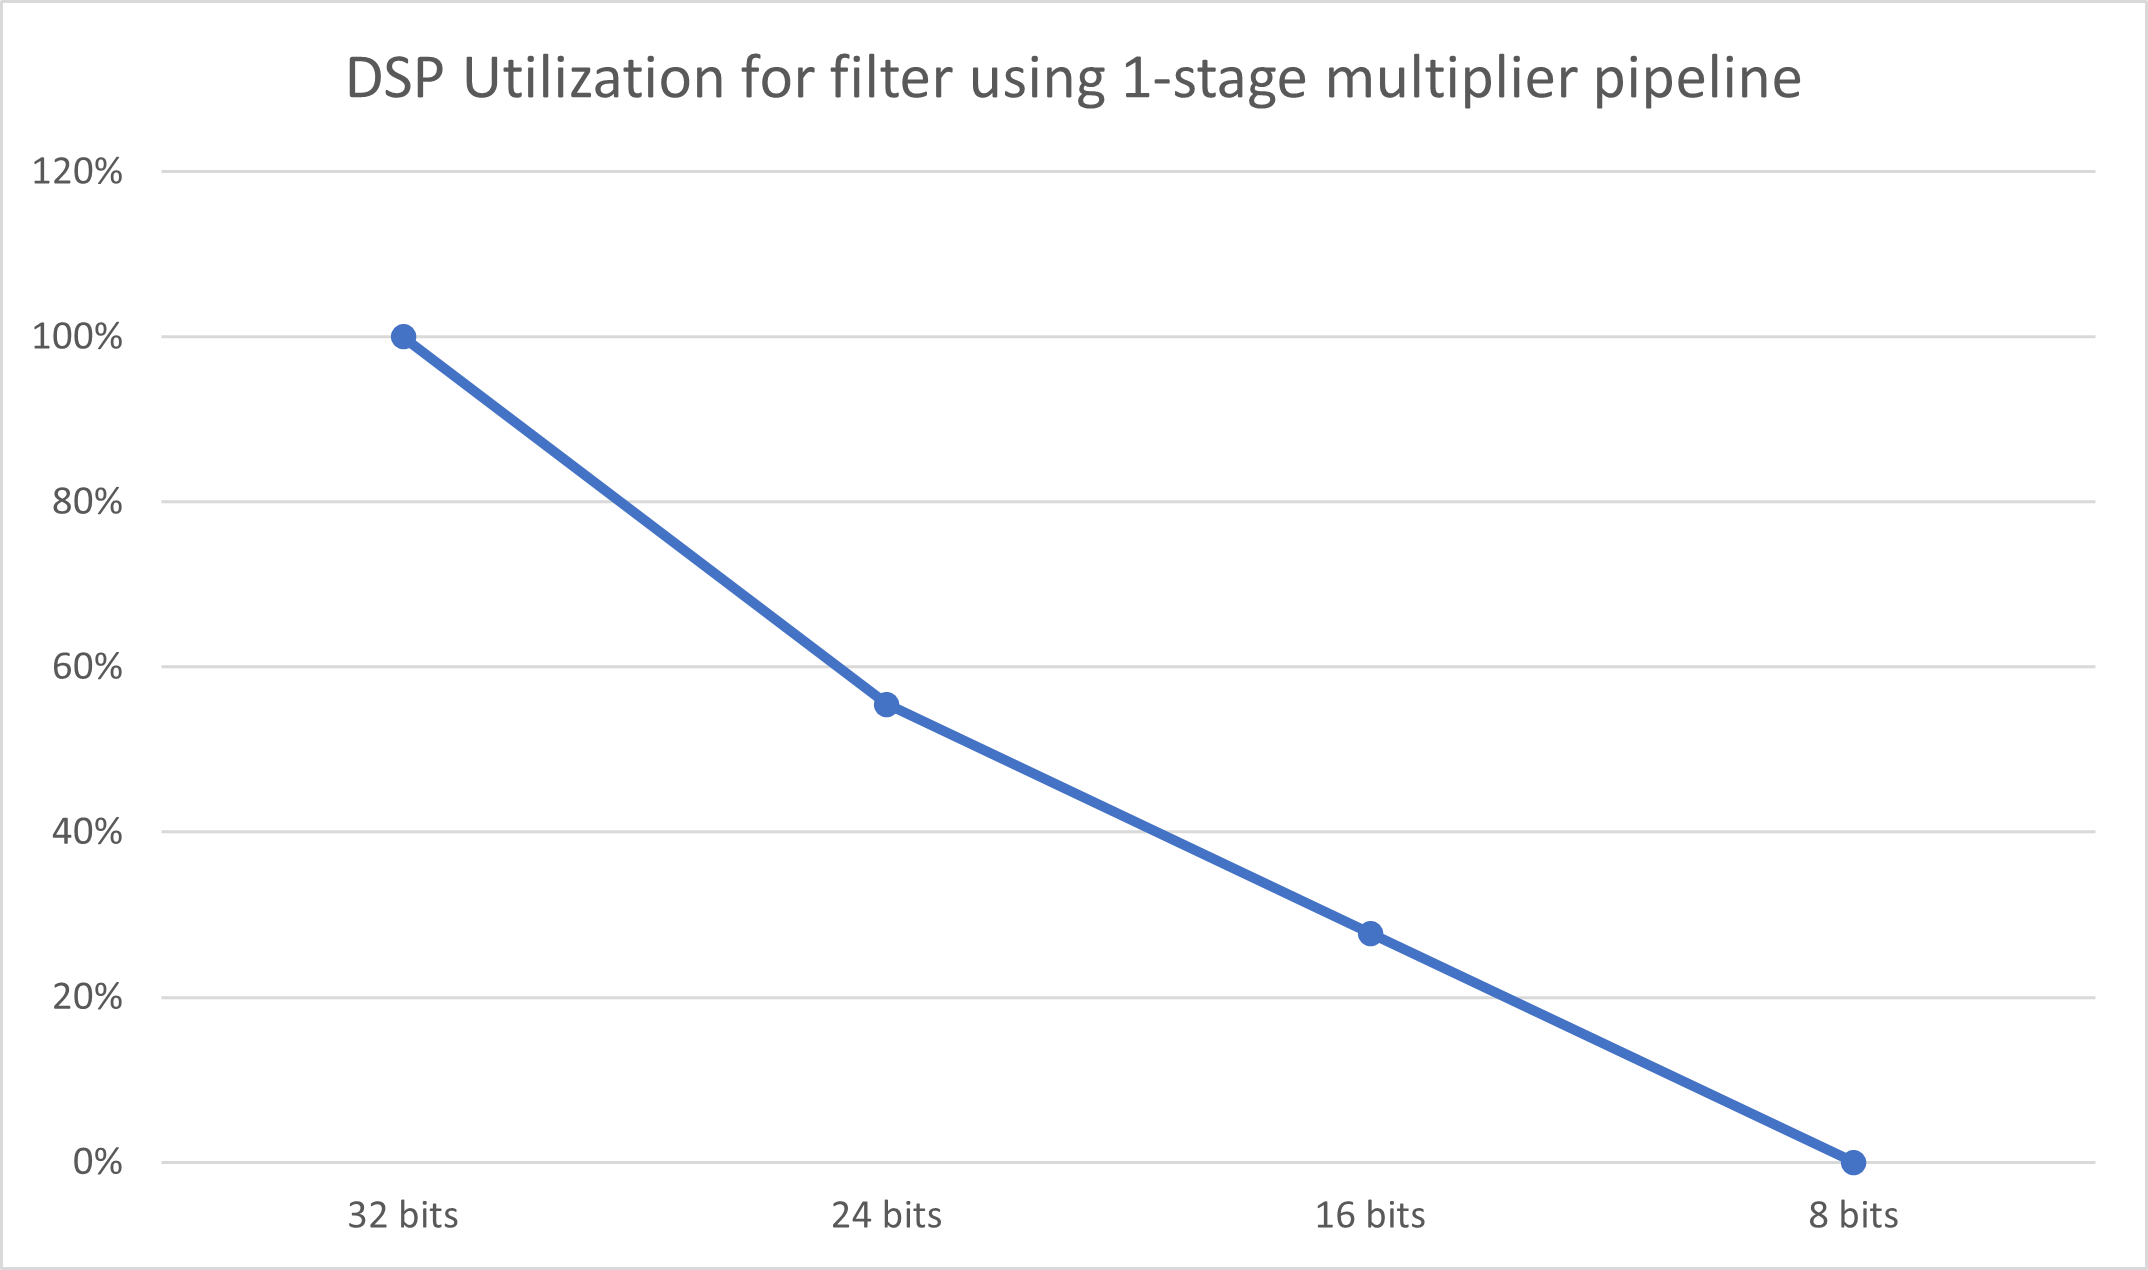
\includegraphics[width=0.45\textwidth]{../Images/FIR_min_Order/multiplier_1_pipeline/dsp_util.png}
	\caption{DSP utilization for min. order filter for different bits}
	\label{fig:fir_min_dsp_util}
\end{figure}

\begin{table}[htbp]
\centering
\begin{tblr}{|c|c|}
	\hline
	Architecture & Time \\
	\hline
	{Multiplier 1-stage pipeline} & 35140 ns\\
	\hline
	{Multiplier 2-stage pipeline} & 35160 ns\\
	\hline
\end{tblr}
\caption{Time for different multiplier pipeline stages using 32 bit floating point arithmetic.}
\label{table:multiplier_stages_time}
\end{table}

Knowing the latency of each architecture, we can calculate the overall execution time for a specific sample set. MATLAB's sample set consists of $3499$ samples. So, using the following formula, we can calculate each architecture's execution time.
\begin{small}
\begin{equation}
	\centering
	\begin{split}
		Execution\hspace{3pt} time &= \\
		& \hspace{-55pt} =\frac{{Latency \hspace{3pt} per \hspace{3pt} sample}\cdot{Number \hspace{3pt} of \hspace{3pt} Samples}}{{Clock \hspace{3pt} frequency}}
	\end{split}
\end{equation}
\end{small}
By inserting numbers in the formula above, we get the diagram that is displayed in fig~\ref{fig:exec_time_latency_min_32}. Clearly, execution time follows the 

\begin{figure}[htpb]
	\centering
	\subfigure[HDL latency for different architectures in samples.]{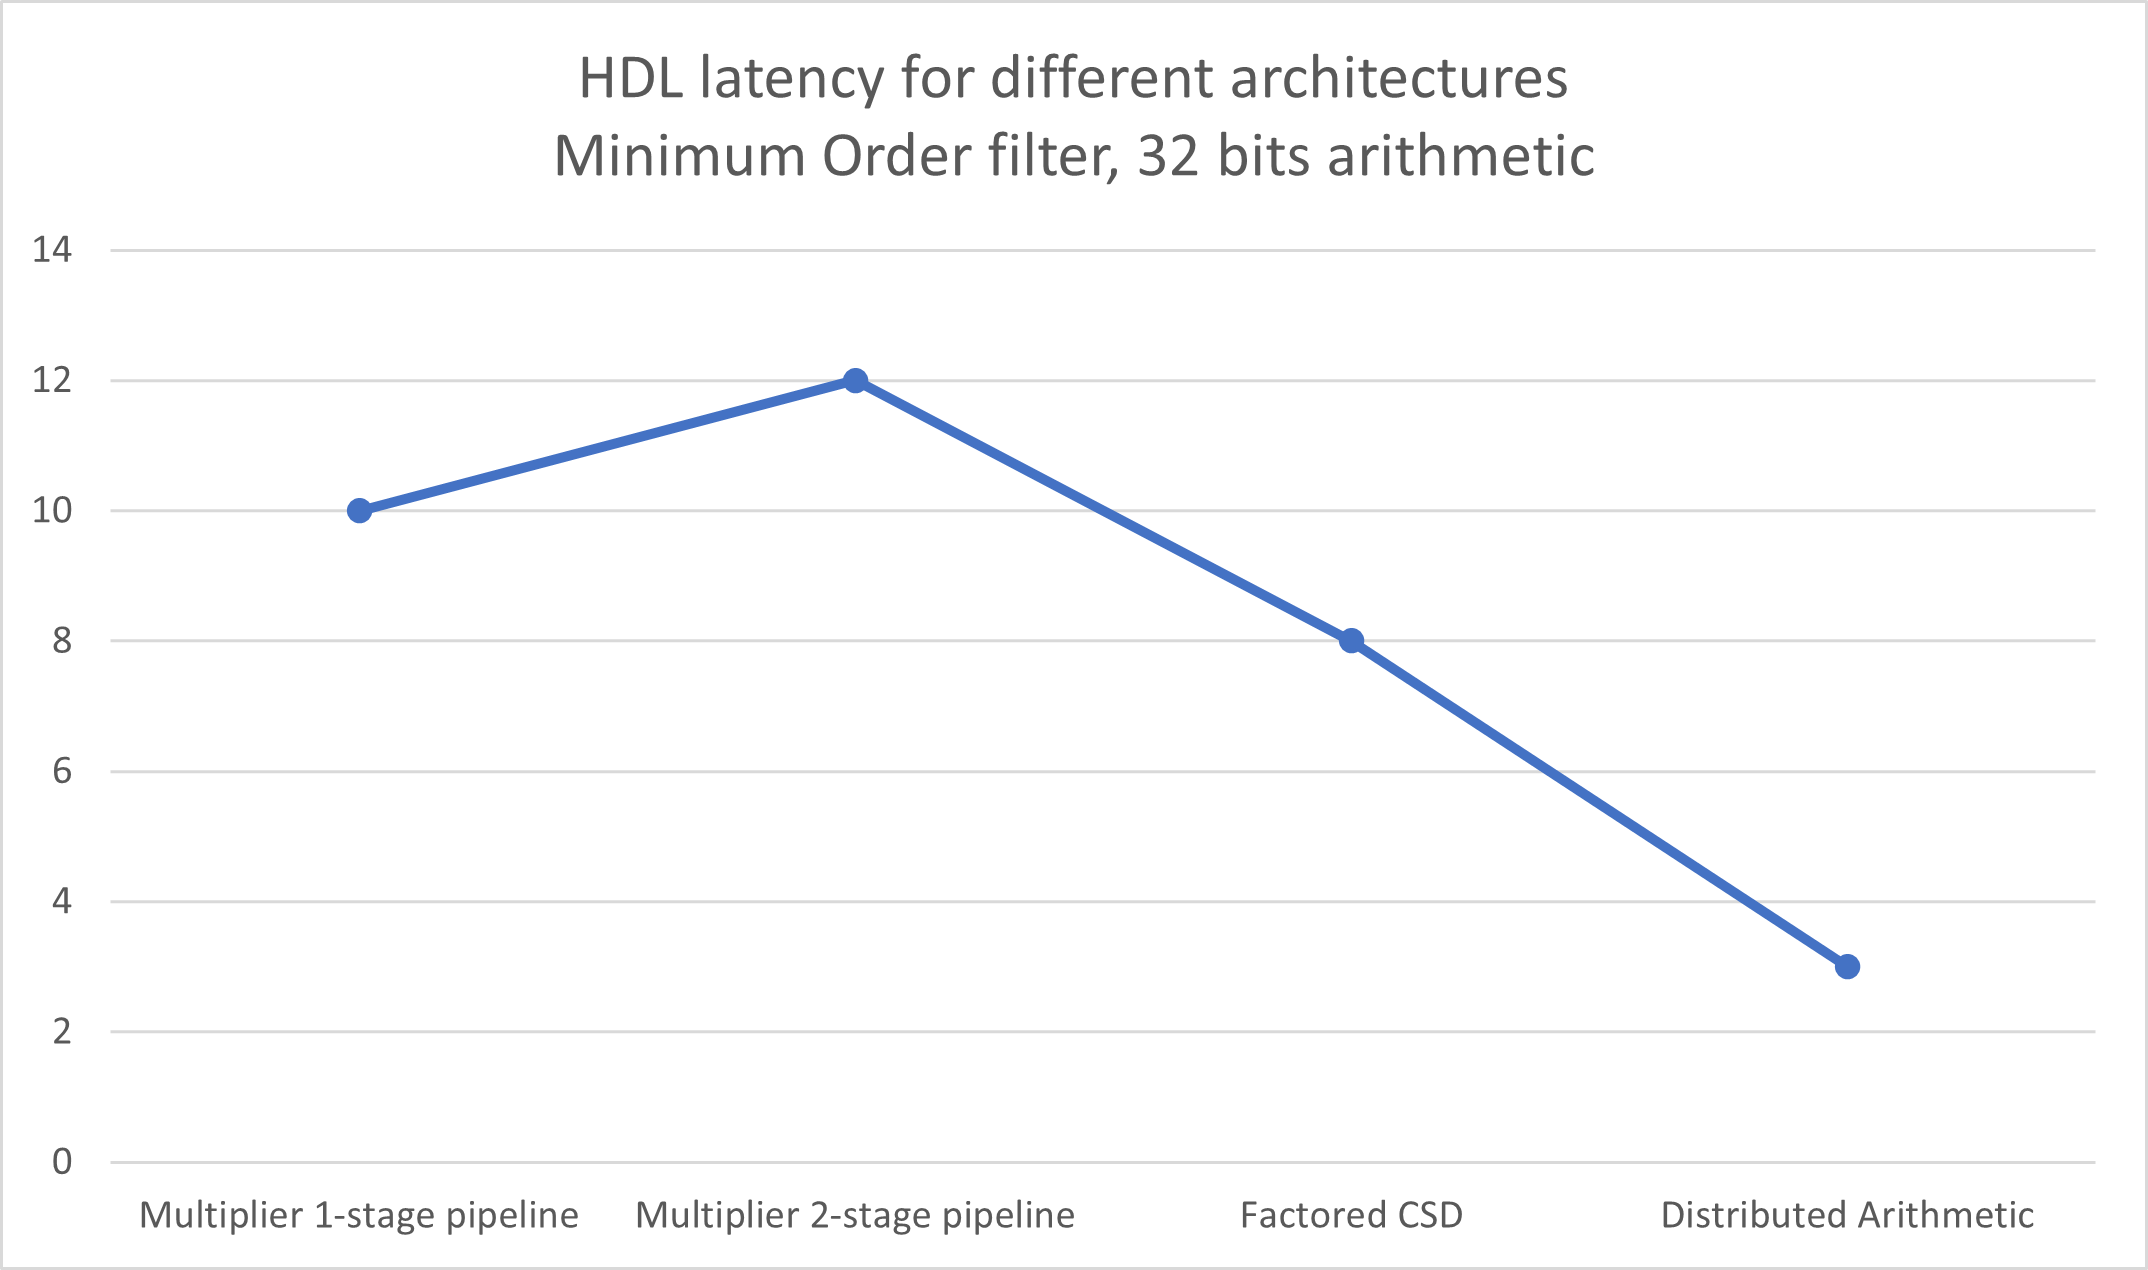
\includegraphics[width=0.45\textwidth]{../Images/FIR_min_Order/hdl_latency_32bits.png}}\\
	\subfigure[Execution time for different architectures in nanoseconds.]{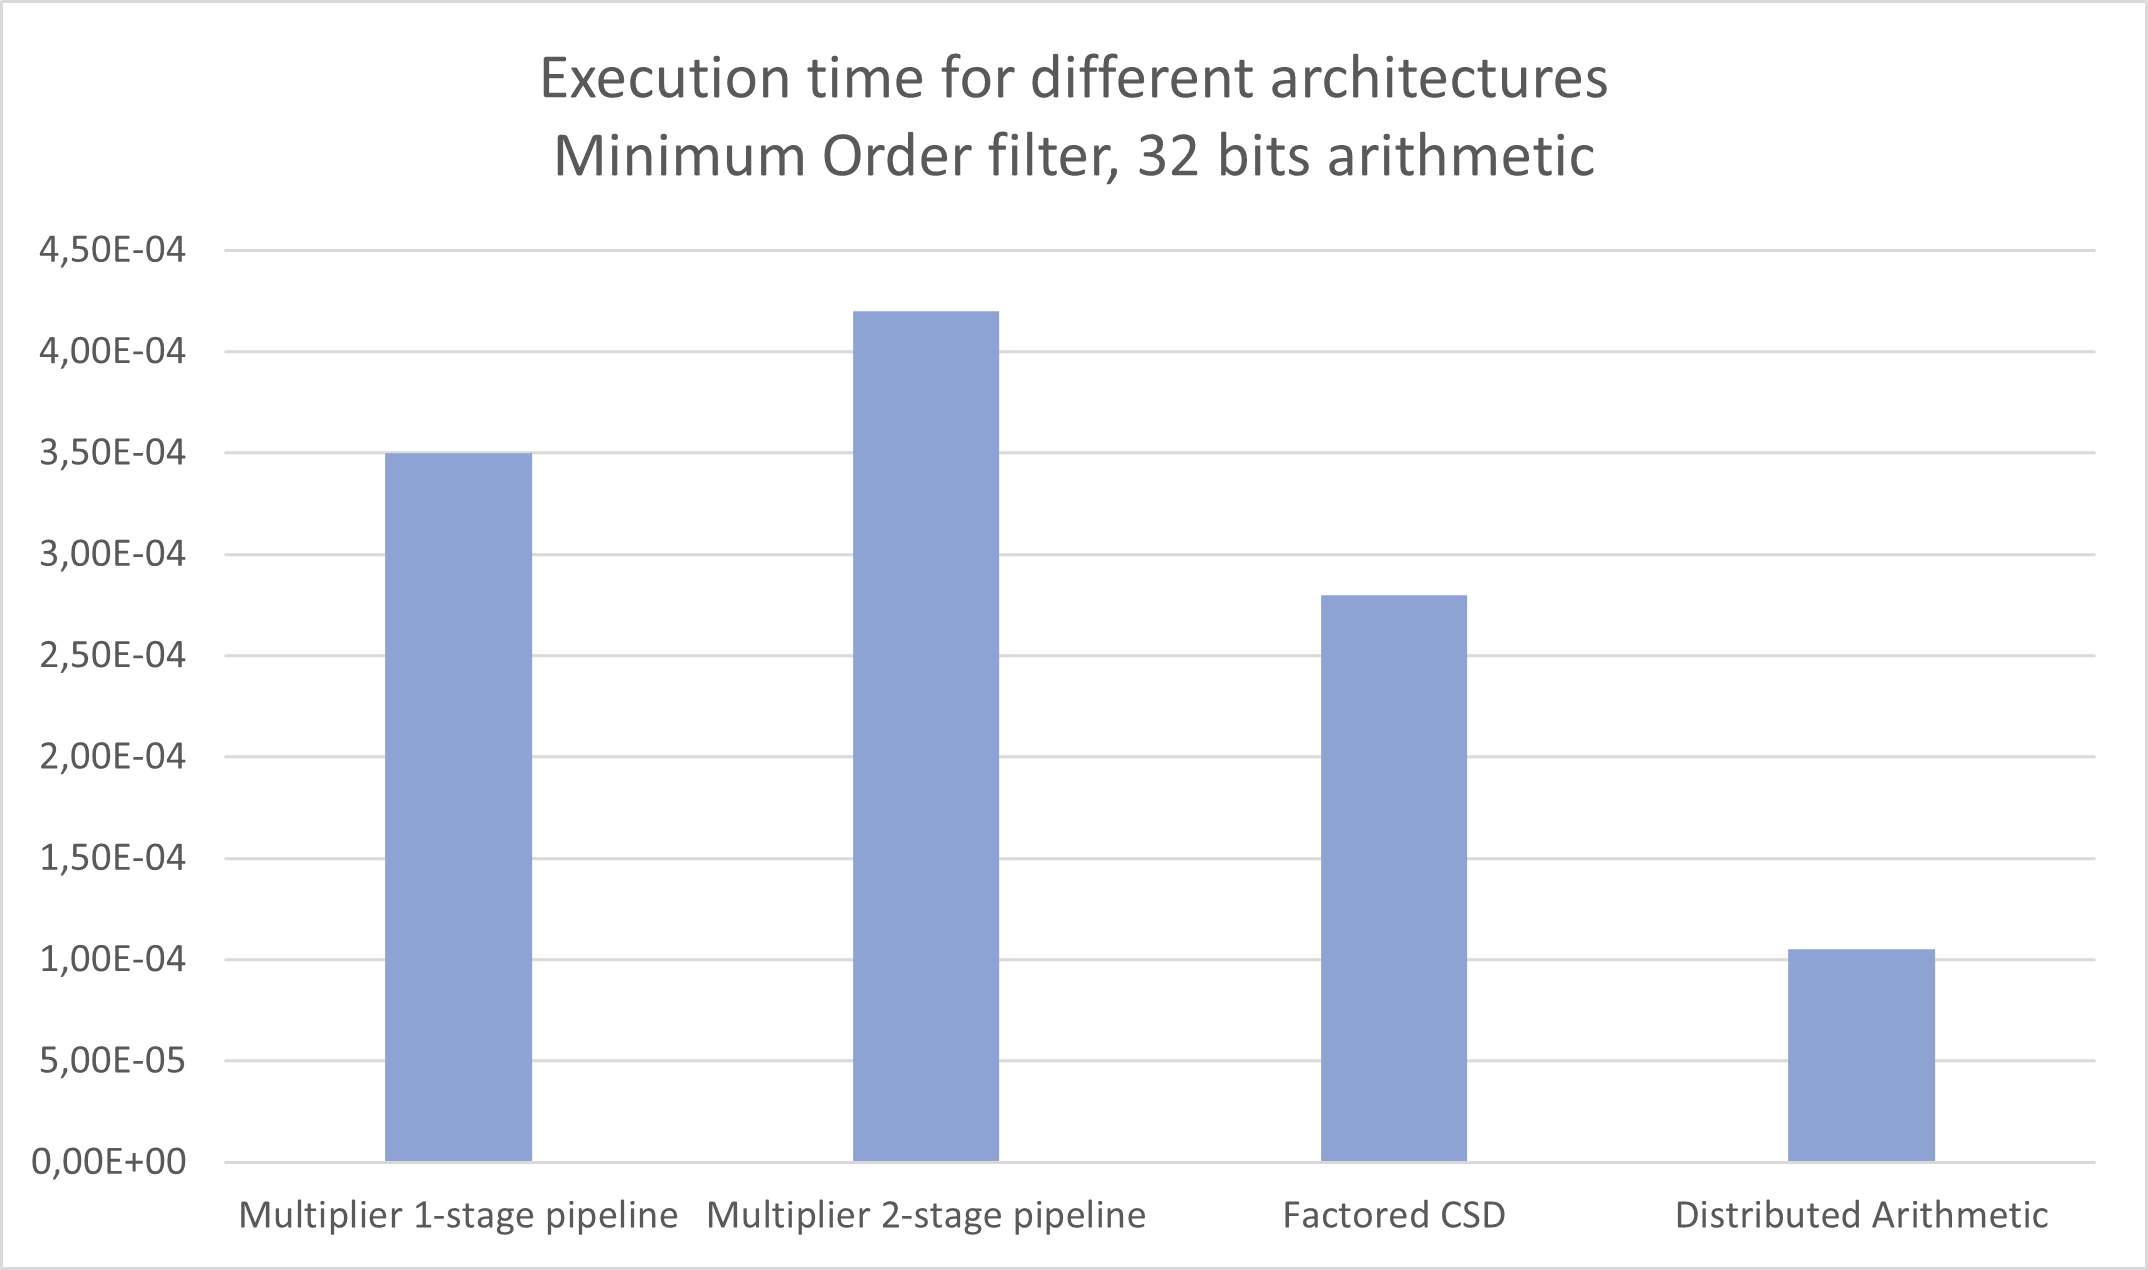
\includegraphics[width=0.45\textwidth]{../Images/FIR_min_Order/exec_time_32bits.png}}
	\caption{Latency and execution time for different architectures.\\ \textit{Note: This is for 32bit arithmetic, the same pattern is observed for the other arithmetics.}}
	\label{fig:exec_time_latency_min_32}
\end{figure}

\subsection{20 Order filter}

\subsection{30 Order filter}

% !TeX spellcheck = en_US

\section{Conclusion}
In conclusion, the architectural differences of the low-pass filter created have been explored in this project.
The 1-stage pipeline multiplier architecture provides a balanced trade-off between complexity and performance. It efficiently processes the input samples in a single pipeline stage, making it suitable for real-time applications where low latency is desired. However, it may require a higher clock frequency to achieve the desired throughput.

The 2-stage pipeline multiplier architecture offers improved performance by dividing the filtering process into two pipeline stages. This allows for better resource utilization and can potentially operate at a lower clock frequency compared to the 1-stage architecture. The 2-stage pipeline multiplier architecture is particularly beneficial when designing filters with a higher order or when implementing resource-constrained systems.

The multiplier-less architecture using factored CSD provides an alternative approach to implementing the low-pass FIR filter. By utilizing CSD coefficients, this architecture eliminates the need for dedicated multipliers, reducing the overall complexity and resource utilization. This approach can be advantageous in applications where hardware resources are limited or power efficiency is a primary concern.

The distributed arithmetic architecture leverages precomputed partial products to perform efficient multiplication operations. It exploits the distributive property of arithmetic operations to minimize the required hardware resources. This architecture is well-suited for implementing low-pass FIR filters with reduced hardware complexity, particularly in applications where area optimization is crucial.

Regarding the bit width configurations, the use of single-precision (32 bits) provides the highest level of precision and dynamic range. However, it comes at the cost of increased computational and memory requirements. Fixed-point representations with lower bit widths, such as 24 bits, 16 bits, and 8 bits, reduce the required resources but introduce quantization effects and potential loss of precision. The appropriate bit width should be selected based on the specific application requirements, considering the trade-off between accuracy and resource constraints.

In conclusion, the architectural differences and bit width configurations of the low-pass FIR filter have a significant impact on its performance, resource utilization, and precision. The choice of architecture and bit width should be carefully considered based on the specific application's requirements, constraints, and trade-offs between accuracy, complexity, power consumption, and resource utilization.
	
\end{document}